\section{External INCART unseen-dataset check}\label{sec:external-incart}

After the final MITDB temporal-holdout system had been fixed, a separate
external check was run on the St Petersburg INCART 12-lead Arrhythmia Database.
This is not the primary thesis benchmark and it is not used for model
selection. It is included to show how the frozen system behaves on an unseen
source database with a different acquisition setting. Lead II is used because
it is the closest practical counterpart to MITDB MLII, but it is not identical
to MLII. Therefore, this section measures both external-patient shift and
lead/device-domain shift.

\begin{figure}[H]
\centering
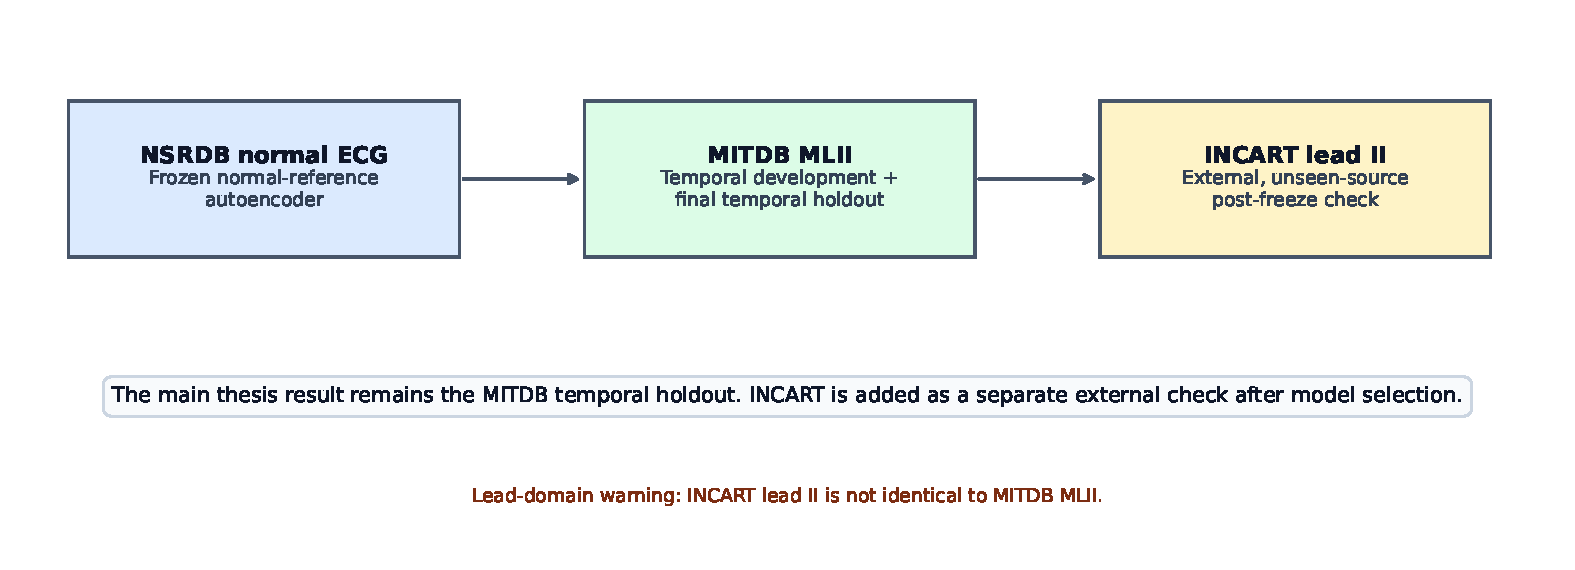
\includegraphics[width=.98\textwidth]{pic/generated/external_incart_protocol.pdf}
\caption{Separation between the main MITDB temporal result and the INCART
external check. The external result is reported after model selection and is
not used to tune the frozen system.}
\label{fig:external-incart-protocol}
\end{figure}

\begin{table}[H]
\centering
\caption{Limited external INCART check on the latest saved evaluation artifact.}
\label{tab:external-incart-summary}
\begin{tabular}{ll}
\toprule
Item & Value\\
\midrule
Dataset & St Petersburg INCART 12-lead Arrhythmia Database\\
Lead and mode & II, offline\\
Records scored & 1 (I01)\\
Annotated beats & 120\\
Saved artifact time & 2026-08-24T09:45:26.627767+00:00\\
Decision threshold & 0.6208\\
Accuracy & 98.33\%\\
Balanced accuracy & 99.10\%\\
Sensitivity / specificity & 100.00\% / 98.20\%\\
Precision / F1 & 81.82\% / 90.00\%\\
AUROC / AUPRC & 1.0000 / 1.0000\\
Confusion counts & TP=9, TN=109, FP=2, FN=0\\
Subtype macro F1 & 0.9691\\
\bottomrule
\end{tabular}
\end{table}

On this limited INCART subset, the frozen hierarchy reached 98.33\%
binary accuracy and 99.10\% balanced accuracy.
All 9 annotated abnormal beats in the subset were detected
and 109 normal beats were rejected, while 2
normal beats were false alarms and 0 abnormal beats were
missed. Because the subset is small and contains only 120
accepted beats from 1 INCART record, this result should be read
as an external sanity check, not as a definitive external clinical validation.

\begin{figure}[H]
\centering
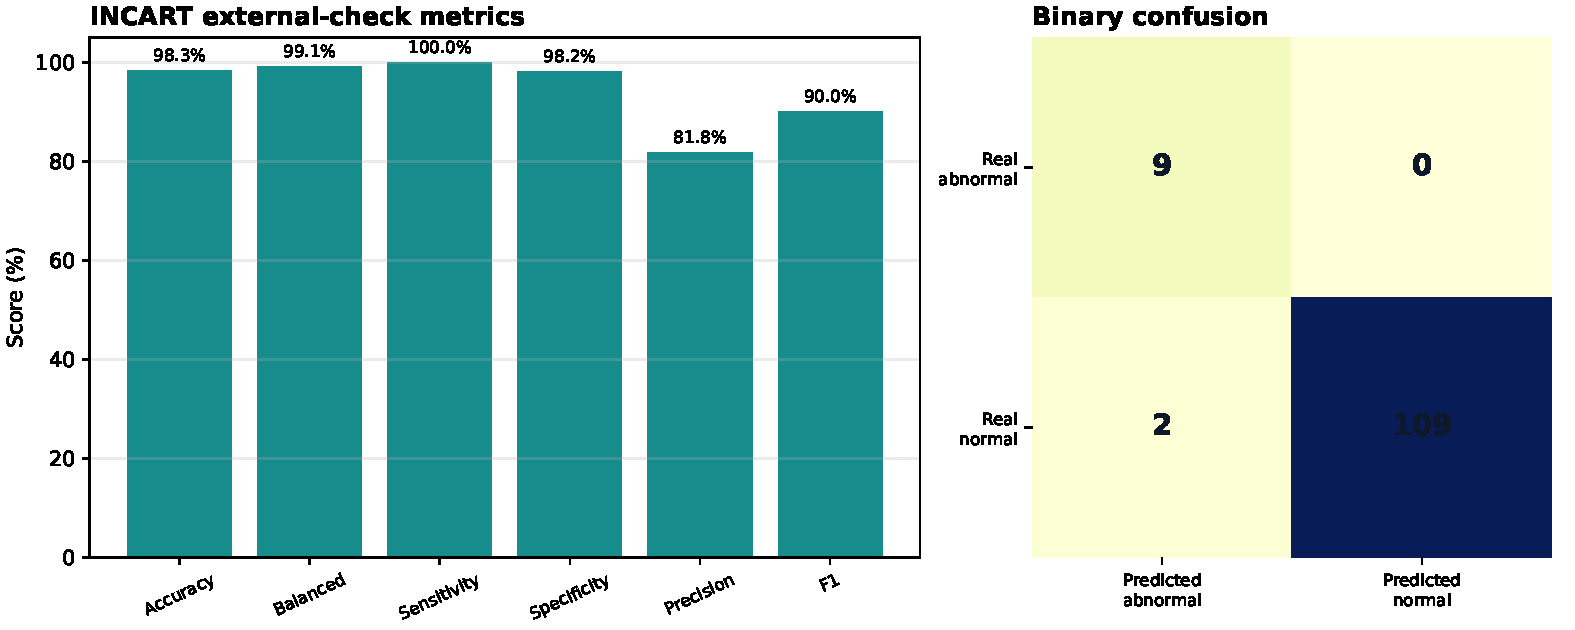
\includegraphics[width=.96\textwidth]{pic/generated/external_incart_metrics_confusion.pdf}
\caption{Metric bars and binary confusion matrix for the limited INCART
external check. Balanced accuracy is shown beside pooled accuracy because the
subset is class-imbalanced.}
\label{fig:external-incart-metrics}
\end{figure}

\begin{figure}[H]
\centering
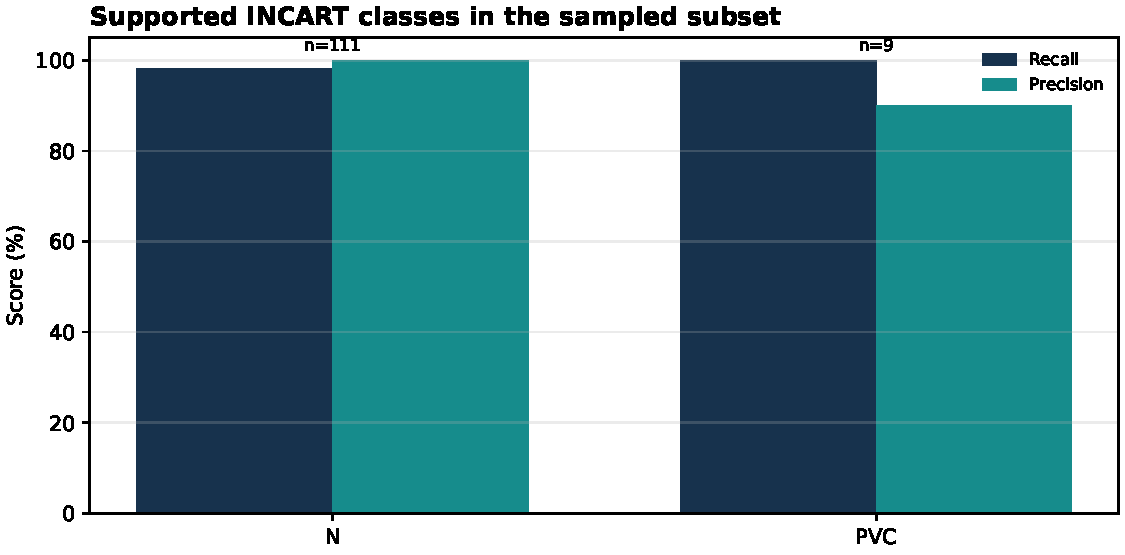
\includegraphics[width=.75\textwidth]{pic/generated/external_incart_class_summary.pdf}
\caption{Class-level precision and recall for classes that appear in the
limited INCART subset. Missing classes are not plotted because they have zero
support in this saved evaluation.}
\label{fig:external-incart-classes}
\end{figure}

\begin{table}[H]
\centering
\caption{Example annotated INCART beats used for visual inspection.}
\label{tab:external-incart-examples}
\begin{tabular}{rllll}
\toprule
No. & Record/sample & Real type & Predicted decision/type & Score\\
\midrule
1 & I01/353 & PVC (V) & Abnormal / PVC & 0.838\\
2 & I01/5426 & PVC (V) & Abnormal / PVC & 0.821\\
3 & I01/4253 & PVC (V) & Abnormal / PVC & 0.750\\
4 & I01/1322 & PVC (V) & Abnormal / PVC & 0.738\\
5 & I01/9029 & PVC (V) & Abnormal / PVC & 0.725\\
6 & I01/9430 & PVC (V) & Abnormal / PVC & 0.717\\
\bottomrule
\end{tabular}
\end{table}

\begin{figure}[H]
\centering
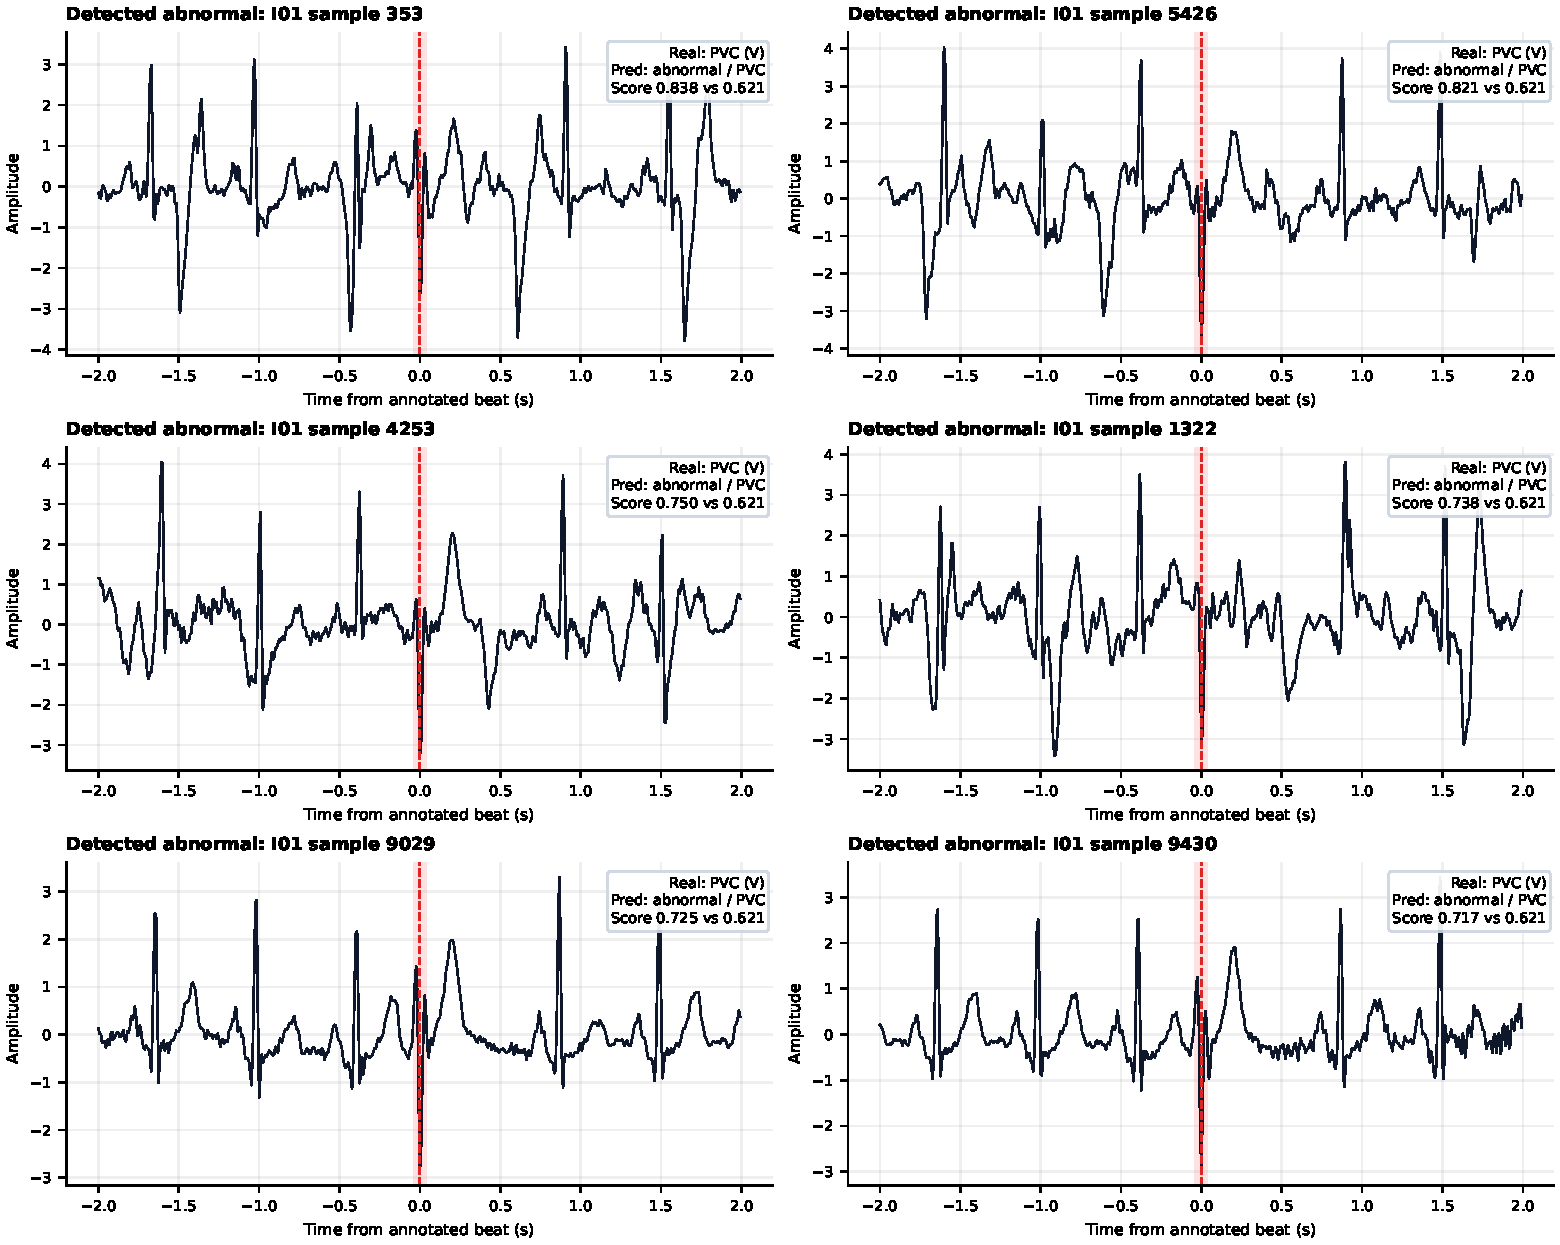
\includegraphics[width=.98\textwidth]{pic/generated/external_incart_examples.pdf}
\caption{Example INCART ECG segments centred on annotated beats. Each panel
shows the real annotation type, the model's abnormal/normal decision, the
predicted anomaly type, and the score-threshold comparison.}
\label{fig:external-incart-examples}
\end{figure}
